\section{Introduction}
Smartwatches have become more and more popular in the consumer market. There are many recently released products such as the Apple Watch \cite{apple-watch}, LG Watch Urbane \cite{lg-urban}, Samsung Gear S \cite{samsung-gear-s}, Sony SmartWatch 3 \cite{sony-sw3}, Pebble Time \cite{pebble-time}, and Moto360 \cite{moto360} that are more powerful and power efficient than ever before and make smartwatches much more capable and practical than prior models. 
Smartwatches rely on small touchscreens and voice recognition for input. Most smartwatches only provide voice input or a selection of predetermined short messages as text entry. Because typing on such a small screen is very difficult with ordinary QWERTY soft-keyboards, a number of solutions to mitigate this problem of text entry on small devices have been proposed. Some of the solution use wristbands, chording, or other sensors  \cite{wristband-text-entry,one-hand-chording,tilt-type,airwriting-on-wearable,mid-air-gesture}, and some work on the design of the keyboard \cite{text-entry-on-small-qwerty,text-entry-for-mobile,zoomboard,1-line-qwerty,splitboard}.

\begin{figure}
  \centering
  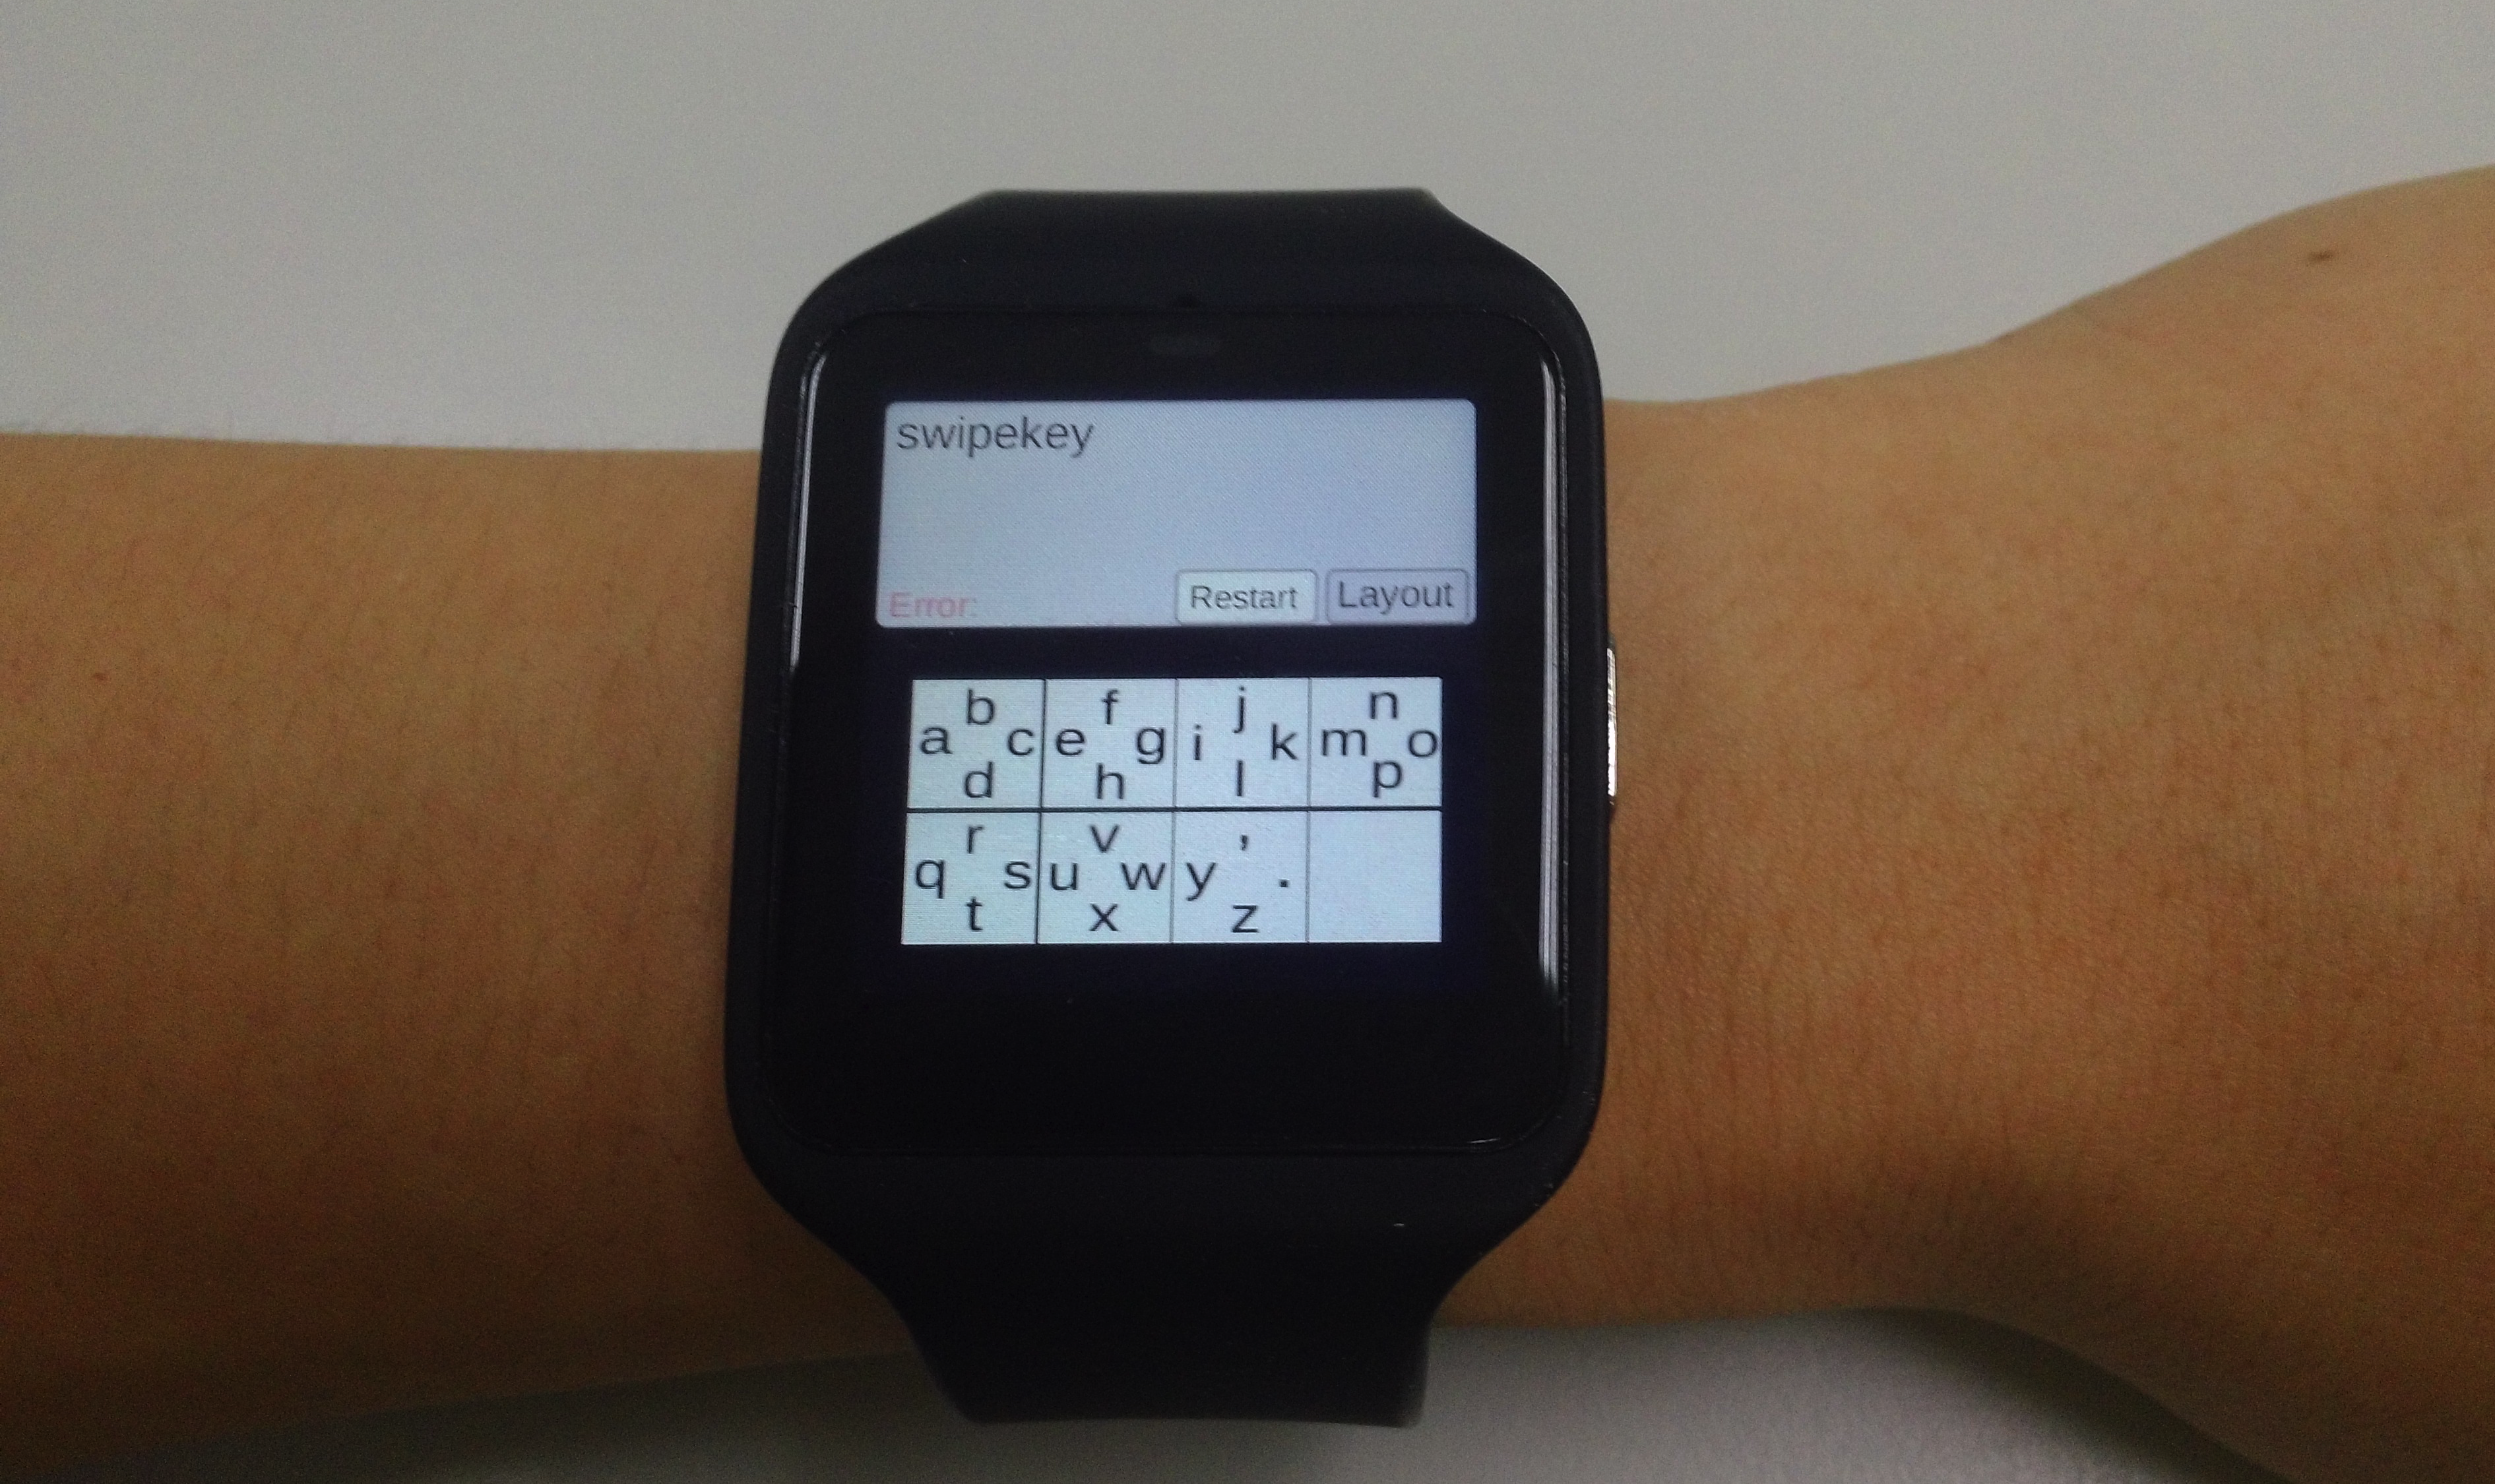
\includegraphics[width=1\columnwidth]{figures/F1.jpg}
  \caption{\papertitle\ 4 implemented on Sony SmartWatch 3}
  \label{fig:f1}
\end{figure}

The major issue for smartwatch text entry is the difficulty of using these extremely small screens for touch input. For example: an iPhone 4 has a screen size of 76.65mm x 51.60mm, the Sony SW3 smartwatch has a screen dimension of 28.7mm x 28.7mm. The dimensions of the onscreen keyboard on an iPhone 4 are 51.6mm x 33.5mm, which is still much larger than the entire screen size of the Sony SW3 smartwatch. Furthermore, we cannot reserve the entire screen of the smartwatch to display a software keyboard since it will leave no space to display text as the user is typing. If we fill half of the smartwatche's screen to display an iPhone 4 software keyboard, each of the keyboard buttons would be 4.2 times smaller on the Sony SW3. A tiny keyboard and button size decreases the users input speed and accuracy when the user is typing on a smartwatch keyboard.

When we talk about the “effective” button size, we mean the ease of pressing buttons due to several factors. One factor is size. Obviously, a big button the size of an ordinary computer keyboard is much easier to press than a tiny button that is less than a quarter the size. Buttons that are both small and tightly packed together will also make pressing a specific button difficult. Since smartwatch screens are naturally small, there are few options that would allow for increased button sizes. This is why we need to incorporate other techniques to make the buttons “feel” bigger. Keyboard designers can achieve this by using gestures. Making them “feel” bigger and easier to type makes the “effective” button size bigger without making the buttons physically bigger.

There are a lot of keyboards designated for small screen mobile devices that attempts to increase the effective button size \cite{zoomboard,swipeboard,text-entry-on-small-qwerty}.
They use many different methods to increase the effective size of the keyboard keys.
 However, Luis etal. \cite{text-entry-on-small-qwerty} shows that the proper design for various small-screen mobile can differ for one of them. These works primarily focus on general mobile devices; for smartwatches specifically however, there is still a room to be explored.

In our paper, we focus on designing a keyboard layout that is suitable for most of the commercially available smartwatches. We have designed a keyboard and have optimized and evaluated several parameters crucial for smartwatch keyboard design through our design process and user studies.

Our first contribution is that we implemented \papertitle: a one swipe or tap keyboard for smartwatches. We tried to optimize several crucial parameters and have shown that \papertitle\ can outperform one existing keyboard for small devices in speed, accuracy, learning difficulty, and user preference.

Our second contribution is that we study some of the parameters of keyboard design and touch screen input on smartwatches. We also provide some design principles for keyboards on smartwatches that have proven themselves in our user studies.
